\documentclass[xcolor=table]{beamer}
\usepackage[utf8]{inputenc}
\usepackage[T1]{fontenc}
\usepackage[alf]{abntex2cite}
\usepackage{udesc}
\usepackage{amsfonts,amsmath,amssymb,mathtools}
\usepackage{verbatim}
\usepackage{listings}
\usepackage[ddmmyyyy]{datetime}
\usepackage{hyperref, url}
\usepackage{graphicx}
\usepackage{bussproofs}
\usepackage{multirow}
\usepackage{changepage}
\usepackage{bussproofs}	

\usepackage{svg}
\setsvg{inkscapeexe=inkscape}
\setsvg{inkscapeopt=-z -D}

\newcommand{\uglyphi}{\phi} % mantendo o \phi velho
\renewcommand \phi{\varphi}
\let \emptyset \varnothing

\newcommand{\Ltac}{$\mathcal{L}$\unskip tac}

\graphicspath{{Figuras/}}
\setbeamertemplate{frametitle continuation}{}

% suprimindo warnings do hyperref
\pdfstringdefDisableCommands{%
  \def\\{}%
  \def\texttt#1{<#1>}%
  \def\smallskip{}%
  \def\medskip{}%
}

\renewcommand{\figurename}{Figura}
\renewcommand{\tablename}{Tabela}
\sloppy
\title{Interpretando Efeitos Algébricos por meio de Mônadas}

\author[Karla A S Joriatti]{
    Karla Alexsandra de Souza Joriatti\\\smallskip
    {\scriptsize Universidade do Estado de Santa Catarina \\\smallskip
    \vspace{-2mm}
    \texttt{kjoriatti@gmail.com}\\\medskip
    {Orientador: Dr. Cristiano Damiani Vasconcellos}\\
    {Coorientador: Me. Paulo Henrique Torrens}\\
    }
}

\date{\today}

% \titlegraphic{Apoio:\\\includegraphics[scale=.15,keepaspectratio]{Logo-CNPq.png}}
% \logo{\includegraphics[scale=.05,keepaspectratio]{Logo-Função.png}}

\begin{document}

    \begin{frame}
        \titlepage
    \end{frame}

    \begin{frame}[allowframebreaks]{Sumário}
        \tableofcontents
    \end{frame}

    \section[]{Introdução}
    \begin{frame}{Introdução}
    % \begin{itemize}
    %     \item \textbf{Compilador:}
    %     \begin{enumerate}
    %         \item Tradução de código em linguagem de programação para código em linguagem de máquina
    %         \item Compilação em etapas (\textit{Front-end} e \textit{Back-end})
    %         \item Etapas ligadas por Representações Intermediárias
    %     \end{enumerate}
    % \end{itemize}
\end{frame}
    \begin{frame}{Objetivo}
    \begin{itemize}
        \item O objetivo fundamental deste trabalho é apresentar uma versão de representação funcional intermediária equivalente à proposta por \citeonline{rigon2020inferring}, porém com tratamento de efeitos por meio do uso de mônadas.
    \end{itemize}
\end{frame}

    % efeito algébrico:  abordagem de efeitos computacionais baseada na premissa de que comportamento impuro surge de um conjunto de operações. Tradicionalmente, os efeitos algébricos eram descritos não apenas por um conjunto de operações, mas também por uma teoria equacional que captura suas propriedades. (Matija Pretnar)

    \section[]{Representação Intermediária de Código}
    \begin{frame}{Representação Intermediária de Código}
    \begin{itemize}
        \item Estrutura de dados usada para manter integridade semântica e possibilitar otimizações~\cite{cooper2014}
              \begin{itemize}
                  \item[--] Classificadas de acordo com o nível de abstração
                  \item[--] Muitas vezes aplicadas em sequência
              \end{itemize}
        \item[] \begin{figure}
                  \centering
                  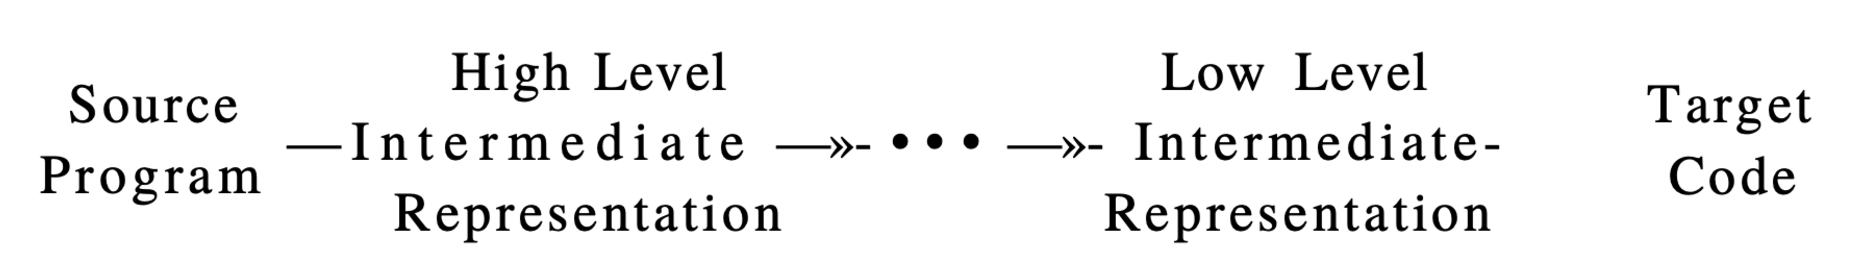
\includegraphics[width=.7\textwidth]{Imagens/abstraction-level-irs.eps}
                  \caption{Sequência de representações intermediárias}\label{fig:abstraction-level-irs}
                  \small{Fonte:~\cite{aho2008compilers}}
              \end{figure}
        \item Fluxo de controle
              \begin{itemize}
                  \item[--] Ordem das instruções
                  \item[--] Escopo
              \end{itemize}
    \end{itemize}
\end{frame}

    \subsection{Grafos de Fluxo de Controle}
    \begin{frame}{Grafo de Fluxo de Controle}
    \begin{itemize}
        \item O grafo de fluxo de controle (\textit{Control Flow Graph}, ou CFG) é uma IR gráfica fundamentada no controle e análise de fluxo de dados.

        \item Modelado como um grafo dirigido $G=(N,E)$, o CFG representa, respectivamente, blocos de código básicos $n$, de forma que $n \in N$, e a transferência de controles de um bloco a outro, modelado como uma aresta $e$, tal que $e \in E$ \cite{allen1970control}.
    \end{itemize}
\end{frame}

\begin{frame}{GFG - Exemplos}
    \begin{figure}
        \centering
        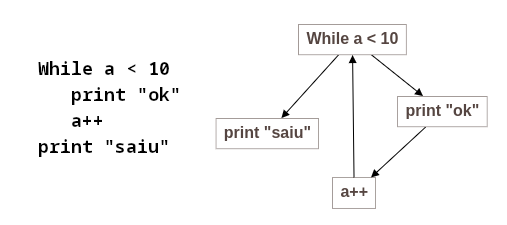
\includegraphics[width=.8\textwidth]{Figuras/cfg.png}
        \caption{Modelagem de \textit{While Statement} em CFG}
        \label{fig:enter-label}
    \end{figure}
\end{frame}

\begin{frame}{GFG - Exemplos}
    \begin{figure}
        \centering
        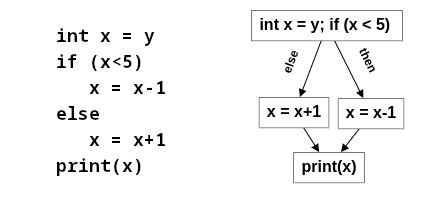
\includegraphics[width=.8\textwidth]{Figuras/cfg2.png}
        \caption{Modelagem de \textit{If Statement} em CFG}
        \label{fig:enter-label}
    \end{figure}
\end{frame}
    \subsection{Atribuição Estática Única}
    \begin{frame}{Atribuição Estática Única}
    \begin{itemize}
        \item A forma de atribuição estática única (do inglês, \textit{static single assignment}, ou SSA) representa uma particularidade de CFG.

        \item Para estar nesse formato, é estabelecido que cada referência a uma variável esteja vinculada a uma única atribuição.

        \item É necessário, então, realizar um procedimento de renomeação de todas as variáveis com mais de uma atribuição no código base.
    \end{itemize}
\end{frame}

\begin{frame}{SSA - Exemplos}
    \begin{figure}
        \centering
        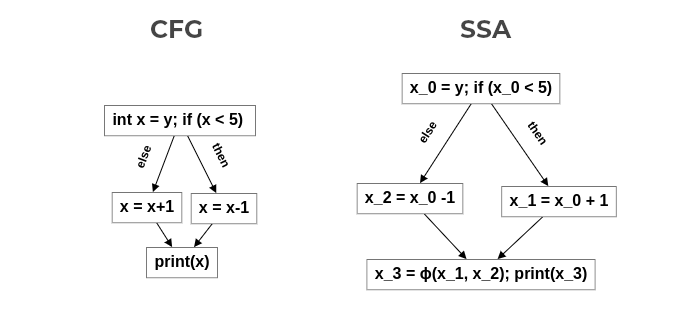
\includegraphics[width=.9\textwidth]{Figuras/ssa-cfg.png}
        \caption{Passagem de CFG para SSA}
        \label{fig:cfg-ssa}
    \end{figure}
\end{frame}

\begin{frame}{Funções $\phi$}
    \begin{itemize}
        \item As funções $\phi$ são funções de decisão que, ao receber como entrada as atribuições provenientes de diferentes arestas que fluem para um mesmo bloco, determinam qual valor utilizar.

        \item Para gerar uma representação SSA eficiente, é necessário que as funções $\phi$ sejam colocadas somente onde são necessárias, pois o excesso destas funções aumenta o custo de qualquer algoritmo que precise percorrer grafo na forma SSA.

        \item Uma estratégia para auxiliar o algoritmo na criação da forma SSA com um número menor de funções $\phi$ é realizar uma análise de dominância entre os blocos.
    \end{itemize}
\end{frame}

\begin{frame}{Análise de Dominância}
    \begin{itemize}
        \item Tabela de dominância: representada por $D_{OM}(n)$, onde $m\in D_{OM}(n)$ se, para alcançar $n$ é \textit{necessário} passar por $m$; e dominante imediato, indicado por $ID_{OM}(n)$, tal que se $m\in D_{OM}(n)$ e $m$ é o nó mais próximo de $n$ neste conjunto, com $m \neq n$, então $m$ é o dominante imediato de $n$. Se $m \in D_{OM}(n)$ e $m\neq n$ então dizemos que $m$ domina estritamente $n$, denotado por $m\gg n$.
        \item[] 

        \item Tabela de Fronteira de Dominância: 
        \begin{equation}
            \begin{matrix}
                DF(n) = \{m | (\exists P \in Pred(m)) & (n \in D_{om}(P) & e & n \not\gg m)\}
            \end{matrix}
        \end{equation}
    \end{itemize}

\end{frame}

    \subsection{Forma A-Normal}
    \begin{frame}{Cálculo Lambda}
    Definido por \citeonline{church1932set}, o cálculo-$\lambda$ puro é representado pela gramática a seguir:

    \begin{flushleft}
        \qquad\qquad M := (M M) \hspace{20ex} (Aplicação)\\
        \qquad\qquad\qquad | V  \\
        
        \qquad\qquad V :=  x  \hspace{26ex} (Variável)\\
        \qquad\qquad\qquad | ($\lambda$x.M) \hspace{20ex} (Abstração)\\
    \end{flushleft}
\end{frame}

\begin{frame}{Cálculo Lambda}
    \begin{itemize}
        \item \textbf{Substituição:} Uma substituição é representada como $M[x:=N]$, de forma que toda ocorrência de $x$ em $M$ será substituída por $N$.

        \item \textbf{$\alpha$-equivalência:} É possível demonstrar a equivalência entre dois termos a partir da mudança de variáveis que estão ligadas em uma abstração, e.g., $\lambda x.x$ $\equiv$ $\lambda y.y$.

        \item \textbf{$\beta$-redução:} ($\lambda$x.M) N := M[x:=N]

        \item \textbf{Contexto:} 
            \begin{enumerate}
                \item \textit{Filling:} seja C = ($\lambda x. y []$) o \textit{filling} C[$\lambda z.x$], é o termo ($\lambda x. y (\lambda z.x)$).
            \end{enumerate}
    \end{itemize}
\end{frame}
    \begin{frame}{Forma A-Normal}
    \begin{itemize}
        \item A forma A-normal (do inglês, \textit{A-normal form}, ou ANF) é uma versão de cálculo-$\lambda$ comumente utilizada como IR.

        \item Um $\lambda$-termo estará em ANF se não puderem ser aplicadas mais reduções do tipo A. \citeonline{sabyr1992} definem o conjunto de reduções A pelas regras:
        \begin{flushleft}
            $(\lambda x.V x) \longrightarrow V  \hspace{21ex} x \not\in FV(V) \hspace{4ex} (\eta_{V})$
            
            $E[((\lambda x.M) N)] \longrightarrow ((\lambda x.E[M]) N)  \hspace{3ex} x \not\in FV(E) \hspace{5ex} (\beta_{lift})$
    
            $E[((M N) L)] \longrightarrow ((\lambda x.E[L]) (M N))  \hspace{2ex} x \not\in FV(E,L) \hspace{3ex} (\beta_{flat})$
    
            $((\lambda x.x) M) \longrightarrow M \hspace{33ex} (\beta_{id})$
    
            $((\lambda x.E[(y x)]) M) \longrightarrow E[(y M)] \hspace{6ex} x \not\in FV(E[y]) \hspace{3ex} (\beta_{\Omega})$
        \end{flushleft}
    \end{itemize}
\end{frame}

    \section[]{Conversão de SSA para Código Funcional}
    \begin{frame}{Conversão de SSA para Código Funcional}
    \begin{itemize}
        \item \citeonline{appel1998ssa} demonstra a equivalência entre código funcional e uma representação na forma SSA

        \item []

        \item [] \begin{figure}
            \centering
            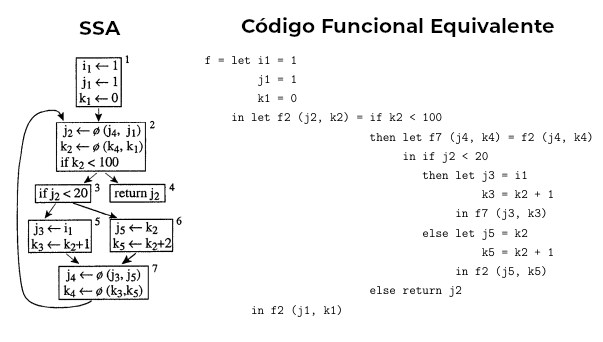
\includegraphics[width=.8\textwidth]{Figuras/ssa-funcional.png}
            \caption{Representações Equivalentes \cite{appel1998ssa}}
            \label{fig:conv1}
        \end{figure}
    \end{itemize}
\end{frame}

    \section[]{Efeitos Colaterais}
    \begin{frame}{Efeitos Colaterais}
    \begin{itemize}
        \item \citeonline{mitchell_2002} define um efeito colateral (\textit{side effect}) como mudanças visíveis no estado da máquina como resultado da valoração de uma expressão.

        \item Duas ocorrências de uma mesma expressão podem ter resultados diferentes

        \item Consequentemente, um beta-redex $(\lambda x.a) b$ é observacionalmente distinto de um beta-reduto $a[x:=b]$ para algum efeito em $b$.
    \end{itemize}
\end{frame}
    \subsection{Mônadas}
    \begin{frame}{Mônadas}
    \begin{itemize}
        \item \citeonline{wadler1995monads} propõe utilizar mônadas como uma forma de simular efeitos colaterais em linguagens funcionais puras.

        \item[] 
        
        \item \textbf{Definição:} \textit{M}, \textit{unit}, $*$

        \item [] \begin{center}
            \textit{unit :: a }$\rightarrow$\textit{ M a}\\
        \end{center}
        \item [] \begin{center}
            \textit{<*> :: M a }$\rightarrow$\textit{ (a }$\rightarrow$\textit{ M b) }$\rightarrow$\textit{ Mb}
        \end{center}

        \item[] 
        
        \item Mônada para erros: data Maybe a = Nothing | Just a
    \end{itemize}
\end{frame}
    \subsection{Sistema de Tipos e Efeitos}
    \begin{frame}{Sistema de Tipos e Efeitos}
    \begin{itemize}
        \item Introduzido por \citeonline{gifford1986integrating}, o Sistema de Tipos e Efeitos é uma extensão de um Sistema de Tipos.

        \item No modelo utilizado por \citeonline{leijen2014koka}, uma sentença possui a forma $\Gamma \vdash e:\sigma | \epsilon$, e uma sentença geral, composta por premissa e conclusão, pode ser definida como:

        \item [] \begin{prooftree}
                \AxiomC{$\Gamma_{1} \vdash e_{1}:\sigma_{1} | \epsilon_{1}$}
                \AxiomC{...}
                \AxiomC{$\Gamma_{n} \vdash e_{n}:\sigma_{n} | \epsilon_{n}$}
                \TrinaryInfC{$\Gamma \vdash e:\sigma | \epsilon $}
            \end{prooftree}

    \end{itemize}
\end{frame}

\begin{frame}{Sistema de Efeitos de Koka}
    \begin{itemize}
        \item \textbf{Koka:} linguagem funcional criada por \citeonline{leijen2014koka}, que utiliza sistema de efeitos.
    
        \item \textbf{Efeitos polimórficos:} o efeito de uma função é determinado a partir dos efeitos de algum de seus argumentos.

        \item [] \begin{center}
            $map : \forall \alpha \beta \mu . (list \langle \alpha \rangle, \alpha \rightarrow \mu \beta) \rightarrow \mu list \langle \beta \rangle$\\
        \end{center}

        \item \textbf{Row-polymorphism:} a combinação de dois efeitos básicos \textit{exn} e \textit{div} gera um \textit{effect-row} $\langle exn, div \rangle$. Por consequência, $\langle exn, exn \rangle \neq \langle exn\rangle$.
    \end{itemize}
\end{frame}

    \section[]{Conversão de Sistema de Efeitos para Mônadas}
    \begin{frame}{Conversão de Sistema de Efeitos para Mônadas}
    \begin{itemize}
        \item A correspondência entre sistema de efeitos e mônadas foi observada por \citeonline{wadler2003marriage}.

        \item Seguindo essa abordagem, \citeonline{vazou2016monads} formalizam a tradução do sistema de efeitos de Koka para mônadas.

        \item[] 

        \item [] \begin{figure}
            \centering
            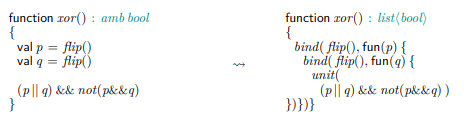
\includegraphics[width=.9\textwidth]{Figuras/conv.png}
            \caption{Exemplo de Tradução da Função \textit{xor} \cite{vazou2016monads}}
            \label{fig:conv1}
        \end{figure}
    \end{itemize}
\end{frame}

\begin{frame}{Conversão de Sistema de Efeitos para Mônadas}
    \begin{itemize}
        \item Para lidar com polimorfismo, cada função que utiliza efeitos polimórficos recebe um dicionário como argumento extra. O dicionário vai encontrar e retornar as funções de \textit{unit} e \textit{bind} correspondentes ao efeito gerado.

        \item Nos casos onde existe a necessidade de traduzir uma função com mais de um efeito (\textit{row-effects}), uma mônada é criada para representar a junção destes efeitos. Morfismos de \textit{lifting} de cada mônada de efeito para a mônada de junção também são criados.
    \end{itemize}
\end{frame}
    % easter egg = Brian
% \begin{frame}{Exemplo de Conversão de Row-Effect}
%     Digamos que existam dois efeitos \textit{IO} e \textit{amb} já definidos e uma função $f$ cujo efeito gerado é $\langle IO, amb \rangle$. Neste caso, uma mônada \textit{IOamb} e as funções \textit{IO2IOamb} e \textit{amb2IOamb} são criadas, de modo que \textit{IO2IOamb} recebe uma mônada \textit{IO} e retorna uma mônada \textit{IOamb} e \textit{amb2IOamb} recebe uma mônada \textit{amb} e retorna uma mônada \textit{IOamb}.
% \end{frame}

    \section[]{Proposta}
    \begin{frame}{Proposta}
    Sistema de tipos monomórfico para CPS com um único construtor (chamado de negação poliádica) para representar continuações \cite{TORRENS2024}:

    \[
        \textit{Types } \ \tau \ ::= \ \neg \vec{\tau} \ \mid \ X
    \]
    \[
        \textit{Environments } \ \Gamma ::= \cdot \mid \Gamma, x : \tau
    \]

    \[
        \frac{
            \Gamma(k) = \neg \vec{\tau}
            \quad \quad
            \Gamma(\vec{x}) = \vec{\tau}
        }{
            \Gamma \vdash k\langle \vec{x} \rangle
        } \quad (J)
    \]

    \[
        \frac{
            \Gamma, k : \neg \vec{\tau} \vdash b
            \quad \quad
            \Gamma, \vec{x} : \vec{\tau} \vdash c
        }{
            \Gamma \vdash b \{ k \langle \vec{x} \rangle = c \}
        } \quad (B)
    \]

    \begin{itemize}
        \item Propor uma extensão ao sistema de tipos
              \begin{itemize}
                  \item[$\blacktriangleright$] Suporte a tipos polimórficos
                  \item[$\blacktriangleright$] Algoritmo de inferência de tipos
              \end{itemize}
    \end{itemize}
\end{frame}

    \begin{frame}{Cronograma}
    % Para o TCC2 as seguintes etapas ficam definidas:
    % \begin{enumerate}
    %     \item Formalização da tradução de código funcional com sistema de efeitos para mônadas
    %     \item Implementação da tradução formalizada na segunda etapa
    %     \item Análise dos resultados
    %     \item Escrita do texto
    % \end{enumerate}
    % \begin{table}[htp]
    %     \centering
    %     \noindent \begin{tabular}{|c|c|c|c|c|c|c|c|}
    %         \hline
    %         \multirow{2}{*}{\textbf{\small{Etapas}}} & \multicolumn{1}{|c|}{\textbf{\small{2023/1}}} &
    %         \multicolumn{5}{|c|}{\textbf{\small{2023/2}}} \\
    %         \cline{2-7}
    %         &\textbf{Dez} & \textbf{Fev} & \textbf{Mar} & \textbf{Abr} & \textbf{Mai} & \textbf{Jun} \\
    %         \hline
    %         \textbf{\small{1}}  & \cellcolor{gray} & \cellcolor{gray} & \cellcolor{gray} & & & \\
    %         \hline
    %         \textbf{\small{2}}  & & \cellcolor{gray} & \cellcolor{gray} & \cellcolor{gray} & & \\
    %         \hline
    %         \textbf{\small{3}}  & & & \cellcolor{gray} & \cellcolor{gray} & \cellcolor{gray} & \\
    %         \hline
    %         \textbf{\small{4}}  & & & \cellcolor{gray} & \cellcolor{gray} & \cellcolor{gray} & \cellcolor{gray}\\
    %         \hline
    %         \end{tabular}
    %     \caption[Cronograma Proposto para o TCC2]{Cronograma Proposto para o TCC2}
    %     \label{tab:cronograma}
    % \end{table}
\end{frame}


    \section[]{Referências}
    \begin{frame}[allowframebreaks]{Referências}
        \bibliography{referencias}
    \end{frame}

\end{document}